\documentclass[aspectratio=169,10pt]{beamer}

% ---------- Theme ----------
\usetheme[progressbar=frametitle,numbering=fraction]{metropolis}
\metroset{titleformat frame=regular}
\metroset{sectionpage=none}
\setbeamertemplate{navigation symbols}{}

% ---------- Packages ----------
\usepackage{graphicx}
\usepackage{xcolor}
\usepackage{booktabs}
\usepackage{array}
\usepackage{listings}
\usepackage[absolute,overlay]{textpos}
\usepackage{tikz}
\usetikzlibrary{positioning}
\usepackage{fontspec}
\setsansfont{Fira Sans}
\setmonofont{Fira Code}[Scale=MatchLowercase]
\usepackage{hyperref}

% ---------- Brand colors ----------
\definecolor{AizaBlue}{HTML}{5D5BFF}
\definecolor{AizaDark}{HTML}{15151A}
\definecolor{AizaMuted}{HTML}{666A73}
\definecolor{CodeBg}{HTML}{F5F6FA}

\setbeamercolor{normal text}{fg=AizaDark,bg=white}
\setbeamercolor{alerted text}{fg=AizaBlue}
\setbeamercolor{frametitle}{fg=AizaDark,bg=white}
\setbeamercolor{progress bar}{fg=AizaBlue,bg=black!12}
\setbeamercolor{title separator}{fg=AizaBlue}
\setbeamercolor{progress bar in head/foot}{fg=AizaBlue,bg=black!12}
\setbeamercolor{section title}{fg=AizaDark,bg=white}

% ---------- Header ----------
\makeatletter
\setlength{\metropolis@progressinheadfoot@linewidth}{1.5pt}
\makeatother
\addtobeamertemplate{frametitle}{}{%
  \begin{tikzpicture}[remember picture,overlay]
    \node[
      anchor=north east,
      xshift=-0.35cm,
      yshift=-0.04cm
    ] at (current page.north east)
    {
\includegraphics[height=0.55cm]{assets/aiza_logo.png}};
  \end{tikzpicture}
}

% ---------- Footer ----------
\setbeamerfont{page number in head/foot}{size=\large}
\setbeamertemplate{footline}{  \hfill
  \usebeamerfont{page number in head/foot}%
  \usebeamercolor[fg]{page number in head/foot}%
  \insertframenumber/\inserttotalframenumber
  \hspace{0.3cm}
  \vspace{0.2cm}
}

% ---------- Code listings ----------

\lstdefinelanguage{Go}{
  morekeywords={package,import,func,type,struct,interface,return,if,else,for,
    range,go,chan,select,case,default,var,const,map,string,int,error,bool,context},
  sensitive=true,
  morecomment=[l]{//},
  morecomment=[s]{/*}{*/},
  morestring=[b]",
}

\lstset{
  language=Go,
  basicstyle=\ttfamily\footnotesize,
  keywordstyle=\color{AizaBlue}\bfseries,
  commentstyle=\color{AizaMuted}\itshape,
  stringstyle=\color{AizaDark},
  backgroundcolor=\color{CodeBg},
  frame=single,
  rulecolor=\color{black!10},
  framerule=0.4pt,
  breaklines=true,
  breakatwhitespace=false,
  columns=flexible,
  keepspaces=true,
  showstringspaces=false,
  tabsize=2,
  xleftmargin=0.6em,
  xrightmargin=0.6em,
  aboveskip=0.6em,
  belowskip=0.1em,
  escapeinside={(*@}{@*)},
}

% ---------- Metadata ----------
\title{Nightmare Navigator}
\subtitle{Building a Horror Movie Telegram Bot in Go}
\author{Angela Scherer}
\institute{CEO/Founder and Software/DevOps Engineer at Aiza GmbH}
\date{Bärner Go X Elastic Talks 2026 no. 2 at Open Systems}

\begin{document}

% ── Title slide ────────────────────────────────────────────────────────────
\begin{frame}[plain]
  \begin{tikzpicture}[remember picture,overlay]
    \node[anchor=north east,xshift=-0.4cm,yshift=-0.35cm] at (current page.north east)
      {
\includegraphics[height=1.0cm]{assets/aiza_logo.png}};
  \end{tikzpicture}

  \vspace{1cm}

  {\Huge\bfseries Nightmare Navigator\par}
  \vspace{0.25cm}
  {\Large Building a Horror Movie Telegram Bot in Go\par}

  \vfill
  {\small Angela Scherer\par}
  {\small Bärner Go X Elastic Talks 2026 no. 2 at Open Systems }
\end{frame}

% ── About me ───────────────────────────────────────────────────────────────
\begin{frame}{About me}
  \Large

  Angela Scherer\\
  \vspace{0.3cm}
  \normalsize
  Freelance Software / DevOps Engineer\\
  Founder and CEO of Aiza GmbH\\
  \textcolor{AizaBlue}{aiza.ch} | \textcolor{AizaBlue}{github.com/angelaschereraiza}

  \vspace{0.1cm}

  \begin{itemize}
    \item Software Architecture and Engineering (Golang, C\#, Python, JavaScript)
    \item Bug Fixing and Stabilization
    \item Kubernetes Engineering and Operations
    \item AI Infrastructure and Data Training
    \item Workshops and Training (Golang, Kubernetes, Podman Quadlet, AI)
  \end{itemize}
\end{frame}

% ── Overview ───────────────────────────────────────────────────────────────
\begin{frame}{Talk overview}
  \Large
  \begin{columns}[T,onlytextwidth]
    \column{0.75\textwidth}
    \begin{enumerate}
      \item Register the bot with Telegram
      \item Choose the Go library
      \item Parse flexible queries
      \item Update recommendations on a schedule
      \item Lessons learned
    \end{enumerate}
  \end{columns}
\end{frame}

\section{Registering the bot}

% ── BotFather: create the bot ────────────────────────────────────────────────
\begin{frame}{BotFather: create the bot}
  \begin{columns}[T,onlytextwidth]
    \column{0.50\textwidth}
    \textbf{Flow in Telegram}
    \begin{enumerate}
      \item Open \texttt{@BotFather}
      \item Send \texttt{/newbot}
      \item Choose display name
      \item Choose username ending in \texttt{bot}
      \item Copy the access token
    \end{enumerate}
  \end{columns}
\end{frame}

% ── BotFather: walkthrough ──────────────────────────────────────────────────

\begin{frame}{BotFather: walkthrough}
  \centering
  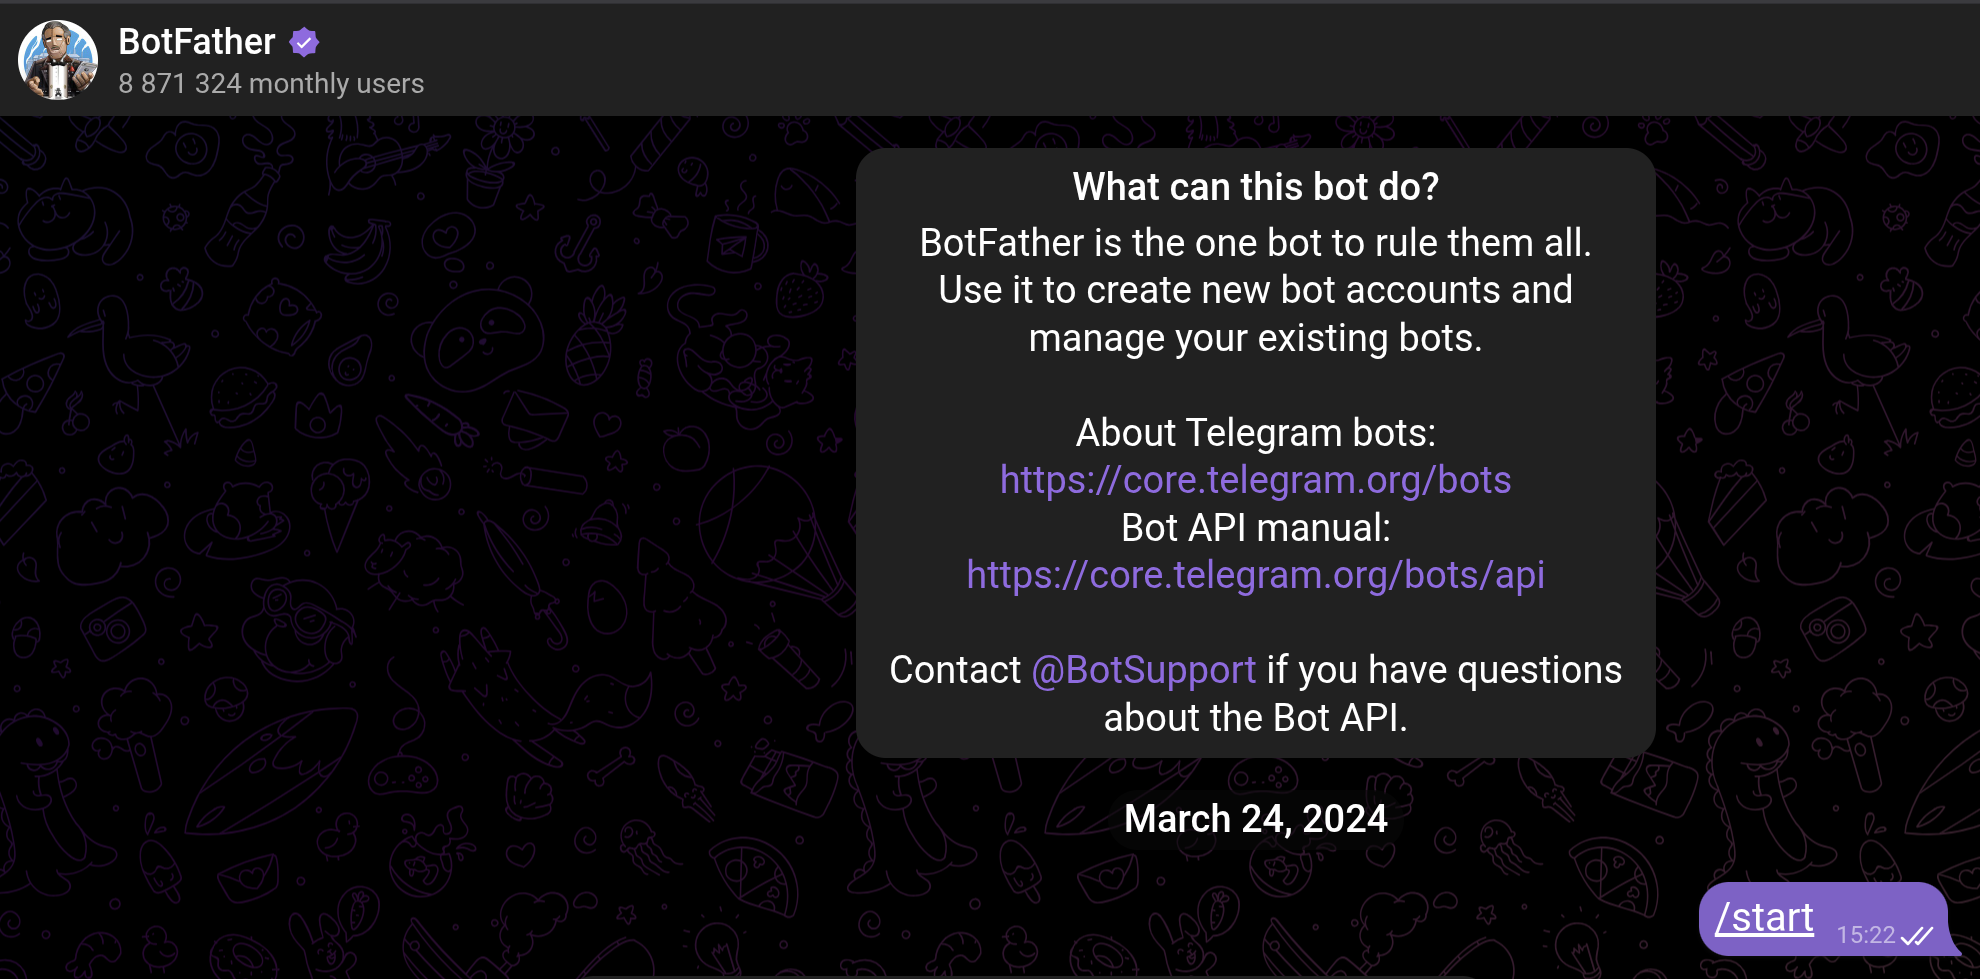
\includegraphics[width=0.9\linewidth]{assets/bot_father_1.png}
\end{frame}

\begin{frame}{BotFather: walkthrough}
  \begin{columns}[T,onlytextwidth]
    \column{0.5\textwidth}
    \centering
    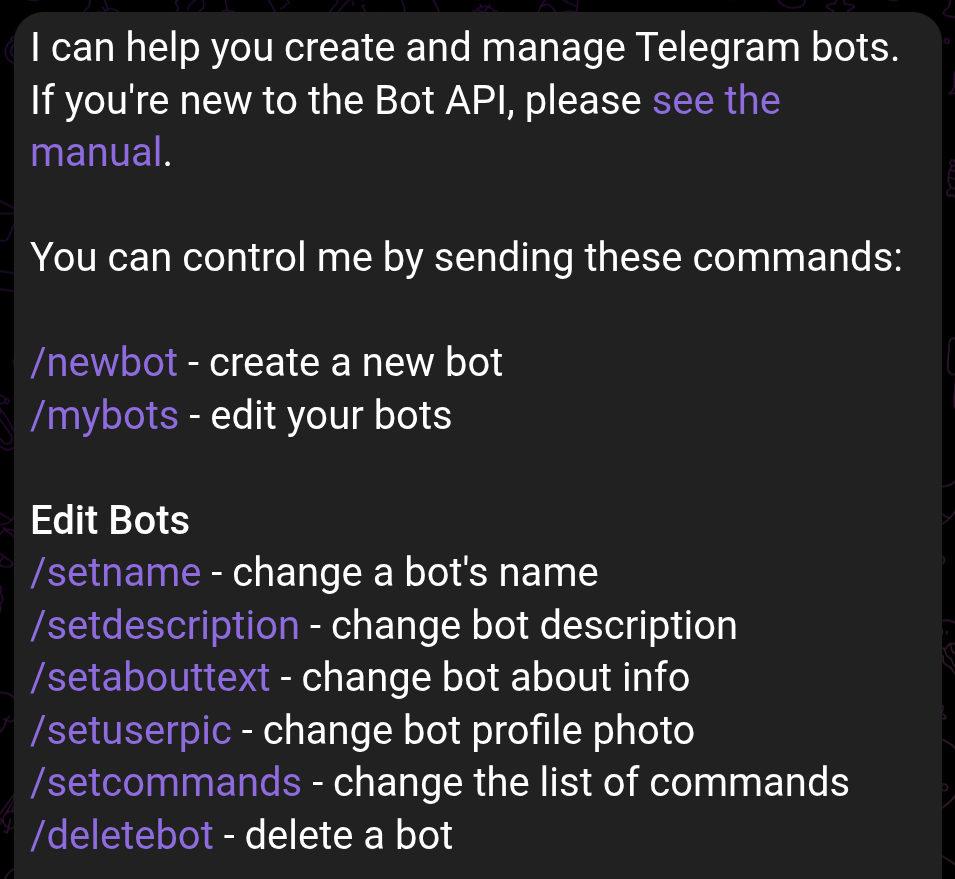
\includegraphics[width=0.9\linewidth]{assets/bot_father_2.png}
    \column{0.5\textwidth}
    \centering
    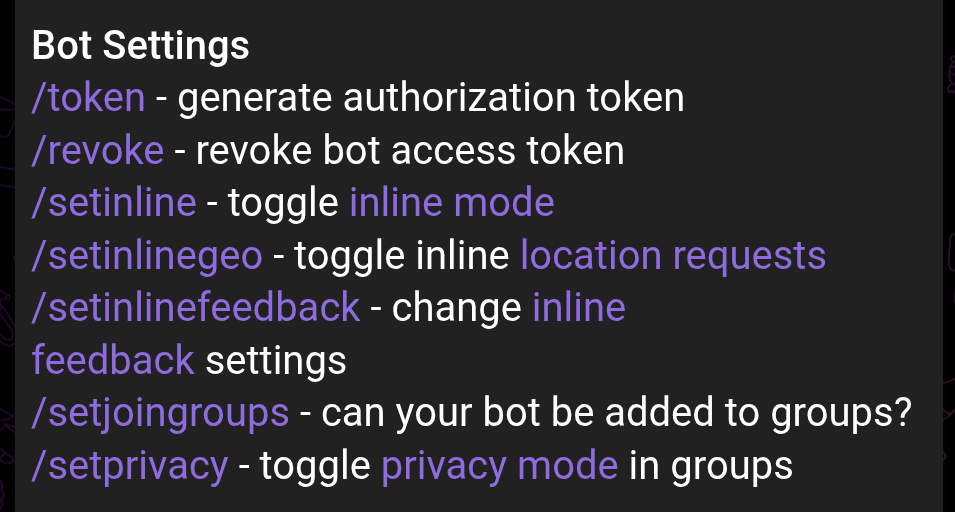
\includegraphics[width=0.9\linewidth]{assets/bot_father_3.png}
  \end{columns}
\end{frame}

\begin{frame}{BotFather: walkthrough}
  \centering
  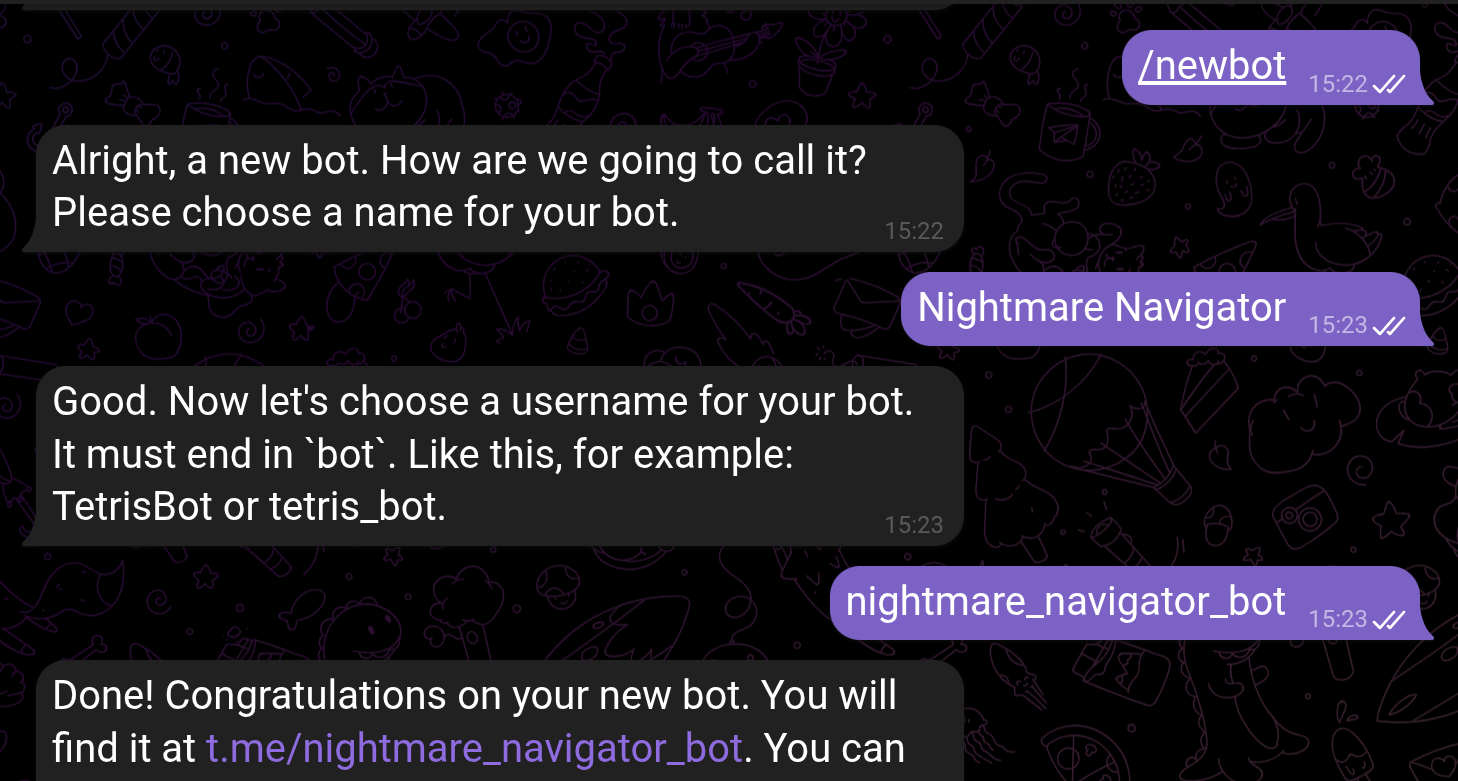
\includegraphics[width=0.9\linewidth]{assets/bot_father_4.png}
\end{frame}

\begin{frame}{BotFather: walkthrough}
  \centering
  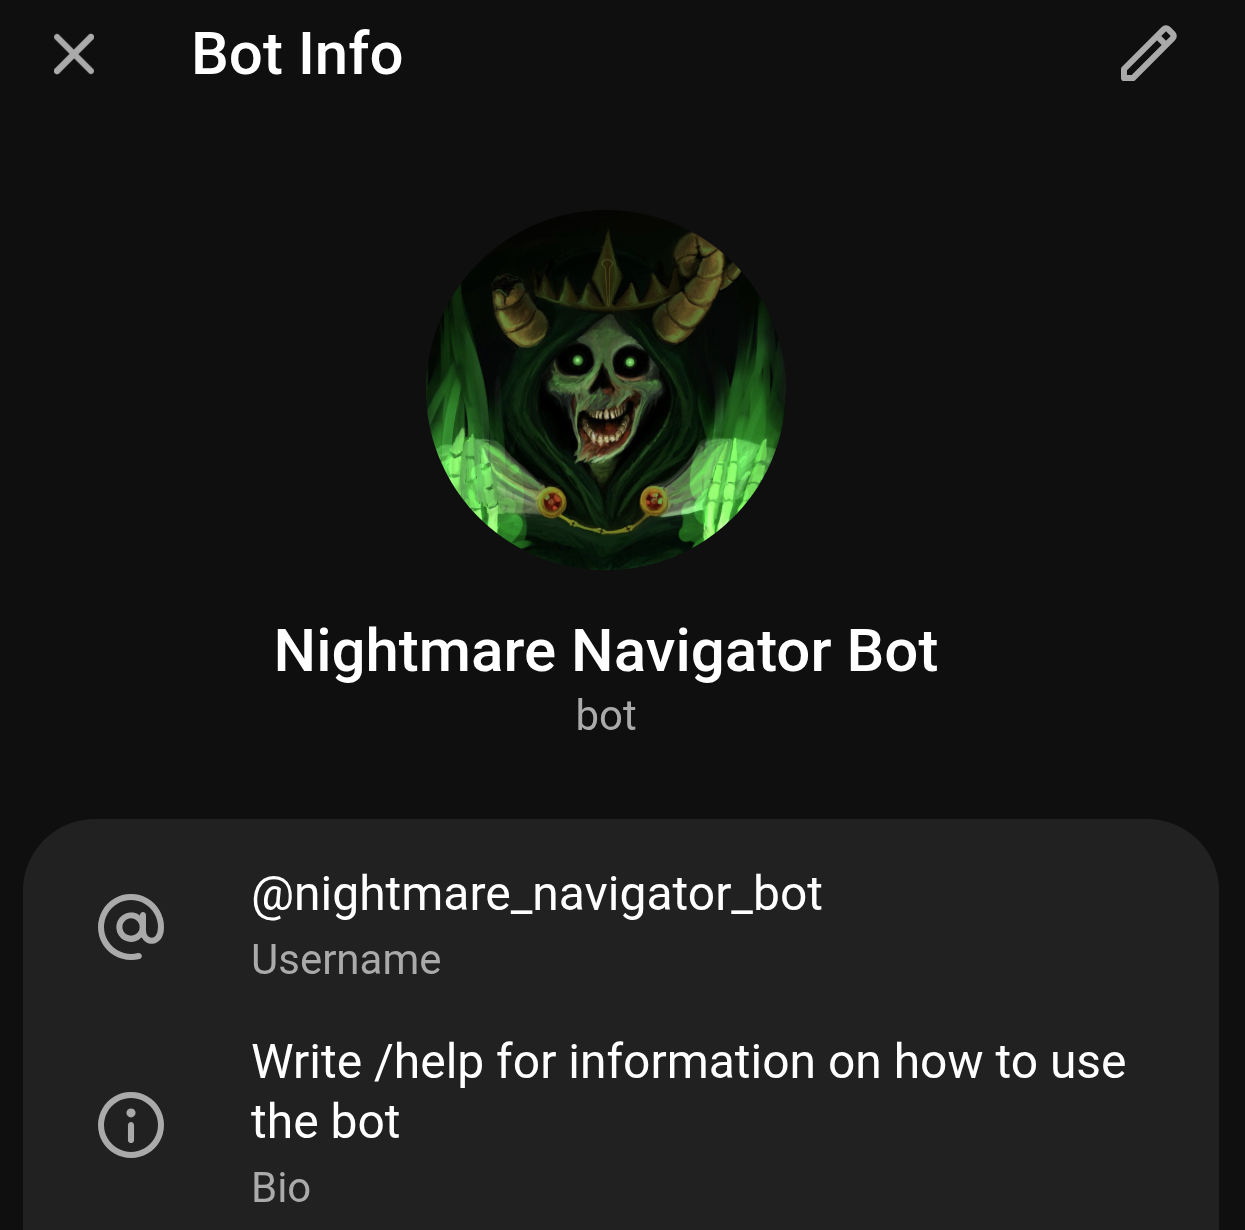
\includegraphics[width=0.5\linewidth]{assets/nightmare_navigator_bot.png}
\end{frame}

% ── Telegram libraries ────────────────────────────────────────────────────

\begin{frame}{Which library?}
  \begin{center}
    \Large
    There are \textbf{50+ Go libraries} for building Telegram bots.

    \vspace{0.5cm}

    \normalsize
    The real choice is not popularity, but abstraction level:\\
    lightweight wrapper or full framework?
  \end{center}
\end{frame}

\begin{frame}{Popular Go Telegram libraries}

\small

{\setlength{\tabcolsep}{5pt}
\begin{tabular}{
  p{0.34\textwidth}
  p{0.49\textwidth}
  p{0.07\textwidth}
}
\toprule
\textbf{Library} & \textbf{Style / strengths} & \textbf{Stars} \\
\midrule

\texttt{go-telegram-bot-api/v5}
&
Minimal wrapper, close to Telegram API, widely adopted
&
~6.4k
\\[4pt]

\texttt{telebot}
&
Framework-like handlers, middleware support, ergonomic API
&
~4k
\\[4pt]

\texttt{gotgbot}
&
Generated API coverage, feature complete, strongly typed
&
~1.5k
\\[4pt]

\texttt{go-telegram/bot}
&
Modern context-based API, lightweight abstraction
&
~1k
\\[4pt]

\texttt{telego}
&
Clean modern design, strong typing, active development
&
~800
\\[4pt]

\texttt{OvyFlash/telegram-bot-api}
&
Maintained fork with newer Telegram Bot API support
&
141
\\

\end{tabular}
}

\end{frame}

\section{Choosing the Telegram library}

\begin{frame}{Why this Telegram library?}
  \Large
  I used \texttt{github.com/OvyFlash/telegram-bot-api}
  because it stays very close to the official Telegram Bot API
  while still being lightweight and easy to use.

  \vspace{0.45cm}
  \normalsize
  \begin{itemize}
    \item Small wrapper around the Telegram Bot API
    \item Less framework abstraction and hidden behaviour
    \item Easy to understand during debugging
    \item Maintained fork with newer Telegram API support
    \item Good fit for a simple command-style bot
  \end{itemize}
\end{frame}

% ── Data sources ───────────────────────────────────────────────────────────
\begin{frame}{Three data sources}
  \Large
  The bot combines multiple movie sources.

  \vspace{0.45cm}
  \normalsize
  \begin{itemize}
    \item \textbf{IMDb datasets}: ratings, vote counts, title IDs and genres
    \item \textbf{The Movie Database}: release dates, runtime and descriptions
    \item \textbf{OMDb}: country and age rating
  \end{itemize}
\end{frame}

% ── Data enrichment ───────────────────────────────────────────────────────
\begin{frame}{Data enrichment flow first version}
  \begin{center}
  \begin{tikzpicture}[node distance=0.85cm, every node/.style={font=\small}]
    \tikzstyle{box}=[draw=AizaBlue, rounded corners, thick, align=center,
                     minimum width=2.65cm, minimum height=0.8cm,
                     fill=AizaBlue!8]

    \node[box] (telegram) {Telegram\\ request};
    \node[box, right=of telegram] (imdb) {Fetch movies\\ from IMDb};
    \node[box, right=of imdb] (tmdb) {Enrich via\\ TMDb};
    \node[box, below=of tmdb] (omdb) {Enrich via\\ OMDb};
    \node[box, left=of omdb] (response) {Telegram\\ response};

    \draw[->, thick, color=AizaBlue] (telegram) -- (imdb);
    \draw[->, thick, color=AizaBlue] (imdb) -- (tmdb);
    \draw[->, thick, color=AizaBlue] (tmdb) -- (omdb);
    \draw[->, thick, color=AizaBlue] (omdb) -- (response);

  \end{tikzpicture}
  \end{center}
\end{frame}

\begin{frame}{Data enrichment flow final version}
  \begin{center}

  \begin{tikzpicture}[every node/.style={font=\footnotesize}]

    \tikzstyle{box}=[
      draw=AizaBlue,
      rounded corners,
      thick,
      align=center,
      minimum width=2.25cm,
      minimum height=0.8cm,
      fill=AizaBlue!8
    ]

    % --- Top row: nightly enrichment ---
    \node[box] (cron) at (0,0) {03:00\\ scheduled job};
    \node[box] (imdb) at (2.9,0) {Fetch movies\\ from IMDb};
    \node[box] (filter) at (5.8,0) {Filter\\ horror movies};
    \node[box] (tmdb) at (8.7,0) {Enrich via\\ TMDb};
    \node[box] (json) at (11.6,0) {Save local\\ JSON cache};

    % --- Bottom row: telegram runtime ---
    \node[box] (telegram) at (0,-2.2) {Telegram\\ request};
    \node[box] (cache) at (5.8,-2.2) {Fetch from local\\ JSON cache};
    \node[box] (omdb) at (8.7,-2.2) {Enrich via\\ OMDb};
    \node[box] (response) at (11.6,-2.2) {Telegram\\ response};

    % --- Top arrows ---
    \draw[->, thick, color=AizaBlue] (cron) -- (imdb);
    \draw[->, thick, color=AizaBlue] (imdb) -- (filter);
    \draw[->, thick, color=AizaBlue] (filter) -- (tmdb);
    \draw[->, thick, color=AizaBlue] (tmdb) -- (json);

    % --- Bottom arrows ---
    \draw[->, thick, color=AizaBlue] (telegram) -- (cache);
    \draw[->, thick, color=AizaBlue] (cache) -- (omdb);
    \draw[->, thick, color=AizaBlue] (omdb) -- (response);

    % --- Cache relationship ---
    \draw[->, dashed, thick, color=AizaMuted]
      (json.south west) -- (cache.north east);

  \end{tikzpicture}

  \end{center}
\end{frame}

% ── Bot runtime ────────────────────────────────────────────────────────────
\begin{frame}[fragile]{The bot runtime}
\begin{lstlisting}
bot, err := tgbotapi.NewBotAPI(cfg.TelegramBot.Token)
if err != nil {
    log.Panic(err)
}

u := tgbotapi.NewUpdate(0)
u.Timeout = 60

updates := bot.GetUpdatesChan(u)
\end{lstlisting}

\vspace{0.25cm}
\begin{block}{Why I like this: }
\vspace{0.1cm}
The code is explicit: receive updates, inspect the message, send a response.
\end{block}
\end{frame}

% ── Main flow ──────────────────────────────────────────────────────────────
\begin{frame}[fragile]{Application startup}
\begin{lstlisting}
cfg, err := config.LoadConfig("config.yaml")
if err != nil {
    log.Fatalf("failed to load config: %v", err)
}

imdbManager := imdb.NewIMDbManager(*cfg)
imdbManager.SaveLatestIMDbRatings()

bot.RunTelegramBot(cfg, imdbManager)
\end{lstlisting}

\vspace{0.25cm}
\normalsize
Startup does three things: load config, refresh movie data, then start listening
for Telegram messages.
\end{frame}

\section{Movie data}

% ── User input ────────────────────────────────────────────────────────────
\begin{frame}{What users can type}
  \Large
  The bot accepts simple, human-ish Telegram messages.

  \vspace{0.45cm}
  \normalsize
  \begin{itemize}
    \item \texttt{movies}
    \item \texttt{15 movies}
    \item \texttt{sci-fi movies}
    \item \texttt{movies 2012}
    \item \texttt{20 sci-fi thriller movies 14.06.19}
  \end{itemize}
\end{frame}

% ── Parsing ───────────────────────────────────────────────────────────────
\begin{frame}[fragile]{Parsing without over-engineering}
\begin{lstlisting}
GetFilteredMovieInfos(
    util.ExtractCount(update.Message.Text),
    util.ExtractGenres(update.Message.Text),
    util.ExtractDate(update.Message.Text),
    imdb.GetIMDbInfosByDateAndGenre,
    BuildMovieInfoStrings,
    *cfg,
)
\end{lstlisting}

\vspace{0.25cm}
\normalsize
Instead of a complex command parser, the bot extracts three things:
count, genres and date.
\end{frame}

% ── Date parsing ──────────────────────────────────────────────────────────
\begin{frame}{Date input}
  \Large
  Dates are intentionally flexible.

  \vspace{0.45cm}
  \normalsize
  \begin{itemize}
    \item Numeric dates: \texttt{14.06.19}, \texttt{14.06.2019}
    \item Year only: \texttt{2012}
    \item Month and year: \texttt{Januar 2012}
    \item Day, month and year: \texttt{01. Januar 2012}
  \end{itemize}

  \vspace{0.25cm}
  If no date is found, the bot uses today.
\end{frame}

\section{Keeping recommendations fresh}

% ── Scheduled refresh ─────────────────────────────────────────────────────
\begin{frame}[fragile]{Daily refresh at 03:00}
\begin{lstlisting}
timer := time.NewTimer(durationUntilNextExecution())

go func() {
    for {
        <-timer.C
        executeAt0300AM(bot, cfg.TelegramBot.GroupId, *imdbManager, *cfg)
        timer.Reset(durationUntilNextExecution())
    }
}()
\end{lstlisting}

\vspace{0.25cm}
\normalsize
The bot refreshes its local movie data and can post newly found movies
automatically to the group.
\end{frame}

% ── Avoiding duplicates ───────────────────────────────────────────────────
\begin{frame}{Avoiding duplicate recommendations}
  \Large
  New movies are tracked in a small JSON file.

  \vspace{0.45cm}
  \normalsize
  \begin{itemize}
    \item Load already returned titles from disk
    \item Filter them out before sending new recommendations
    \item Save the updated list after sending
    \item Keep the behaviour stable across restarts
  \end{itemize}
\end{frame}

\section{Lessons learned}

% ── Lessons learned ───────────────────────────────────────────────────────
\begin{frame}{Lessons learned}
  \begin{itemize}
    \item A simple Telegram wrapper was enough for this project
    \item Most of the value is in data filtering and enrichment
    \item Local JSON cache keeps the bot fast and predictable
    \item Flexible input feels better than strict commands
    \item Scheduled refresh makes the bot useful without manual work
  \end{itemize}
\end{frame}

% ── Demo ──────────────────────────────────────────────────────────────────
\begin{frame}{Demo}
\vspace{0.cm}
\begin{center}
    {\Large Nightmare Navigator in action}

    \vspace{0.1cm}

    
\includegraphics[width=0.4\linewidth]{assets/bot_logo.png}
\end{center}
\end{frame}

% ── Questions ─────────────────────────────────────────────────────────────
\begin{frame}{Questions and discussion}
  \begin{tikzpicture}[remember picture,overlay]
    \node[
      anchor=center,
      xshift=2.1cm,
      yshift=1.2cm
    ] at (current page.center)
    {
      
\includegraphics[width=0.32\linewidth]{assets/question_mark.png}
    };

    \node[
      anchor=center,
      xshift=0cm,
      yshift=-1.85cm
    ] at (current page.center)
    {
      
\includegraphics[width=0.25\linewidth]{assets/gopher.png}
    };

  \end{tikzpicture}
\end{frame}

\end{document}